\documentclass[a4paper,11pt]{article}
\usepackage{latexsym}
\usepackage[polish]{babel}
\usepackage[utf8]{inputenc} 
\usepackage[MeX]{polski}
\usepackage{nicefrac}
\usepackage{listings}
\usepackage{multirow}
\usepackage[normalem]{ulem}
\useunder{\uline}{\ul}{}
\usepackage{float}
%\usepackage[margin=0.6in]{geometry}
\usepackage{graphicx}
\usepackage{multicol}
\lstset{showstringspaces=false}

\author{Marcin Mrugas 122580 \\
		Marcin Drzewiecki 122472}

\title{Przetwarzanie i rozpoznawanie obrazów\\ 
\large{{\bf Sprawozdanie} \\ Projekt 2 -- deskryptor obrazu}} 

\date{20 maja 2018}

\begin{document}

\maketitle 

\section{Metody wyznaczania deskryptora obrazu}

Jeśli nie wskazano inaczej, jako otoczenie punktu należy rozumieć koło o promieniu $ r = 32 $ o środku w danym punkcie.
Przed zastosowaniem metod, na otoczeniu była stosowana normalizacja jasności obrazu, tj. zmiana jasności piksela wg wzoru:

$$ \frac{v_i - min(v)}{max(v)-min(v)},$$
gdzie $v$ -- otoczenie punktu, $v_i$ -- $i$-ty piksel otoczenia.

\subsection{Średnia jasność otoczenia}

\subsubsection{Ekstrakcja}
Najprostsza metoda polegała na wyznaczeniu średniej jasności pikseli w otoczeniu danego punktu.

\subsubsection{Porównanie}
Porównanie deskryptorów polegało badaniu zależności między wyznaczonymi średnimi zgodnie z wzorem:

$$ min(1, \frac{|des_1 - des_2|}{64}) $$

\subsubsection{Wynik działania}

\begin{figure}[H]
\begin{center}
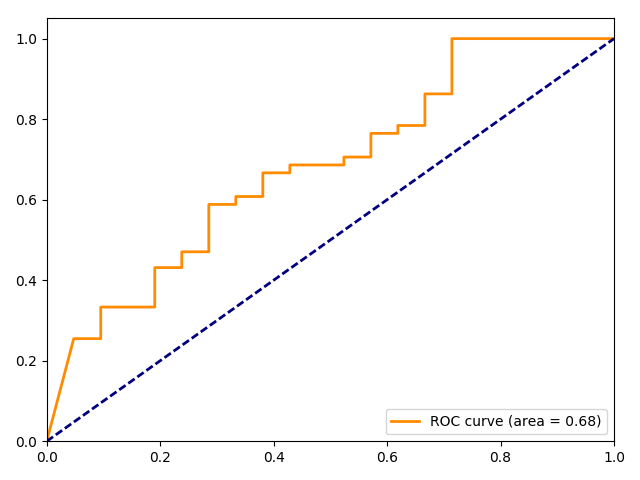
\includegraphics[width=0.7\textwidth]{./img/average.png}
\end{center}
\caption{Wynik działania deskryptora, AUC.}
\end{figure}


\subsection{Momenty Hu}

\subsubsection{Ekstrakcja}
Metoda polegała na wyznaczeniu momentów Hu z otoczenia punktu. 

\subsubsection{Porównanie}
Najpierw wyznaczono dla każdego momentu wartości:
$$ v_i = -sgn(h_i) * log_{10}|h_i|, $$
gdzie $h_i$ oznacza $i$-ty moment Hu, a $sgn(x)$ -- znak liczby $x$.
Następnie porównano dwa wektory $v$ oraz $w$zgodnie ze wzorem:

$$ \sum_{i=1}^{7}|v_i - w_i|$$

\subsubsection{Wynik działania}

\begin{figure}[H]
\begin{center}
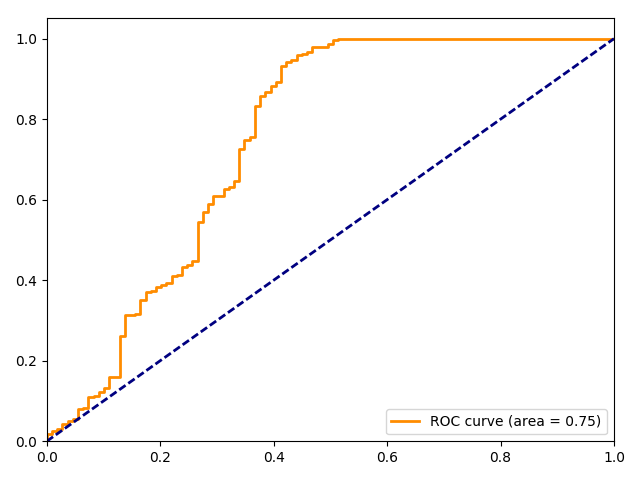
\includegraphics[width=0.7\textwidth]{./img/hu.png}
\end{center}
\caption{Wynik działania deskryptora, AUC.}
\end{figure}

\subsection{Średnie jasności na okręgach}

\subsubsection{Ekstrakcja}
Metoda polegała na wyznaczeniu średniej jasności pikseli oddalonych o $r = 0,1,...,32$ od badanego punktu. 
W ten sposób otrzymano wektor o długości $33$.

\subsubsection{Porównanie}
Dla każdego z współczynników: $a = 0.7, 0.8, 0.9, 1, \frac{1}{0.7}, \frac{1}{0.8}, \frac{1}{0.9}$, wykonywano następujące czynności.
Porównywano pierwsze $\left \lfloor  a \cdot 33 \right \rfloor$ elementów pierwszego wektora oraz tyle samo elementów drugiego wektora. Aby uzyskać odpowiednią długość drugiego wektora dokonywano operacji analogicznej do decymacji w cyfrowym przetwarzaniu sygnałów.
Dzięki temu deskryptor był odporny na skalowanie.
Porównanie dwóch wektorów polegało na wyznaczeniu korelacji ($c_i$) między dwoma wektorami oraz wybranie maksymalnej z wyznaczonych wartości i odjęcie jej od $1$:

$$ 1-max(c) $$

\subsubsection{Wynik działania}

\begin{figure}[H]
\begin{center}
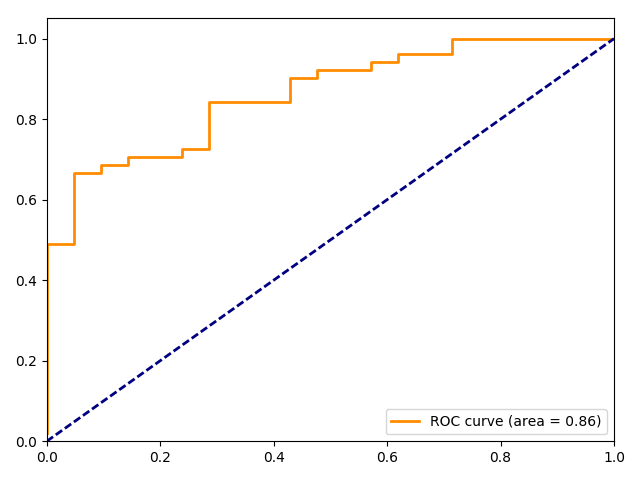
\includegraphics[width=0.7\textwidth]{./img/circle_hist.png}
\end{center}
\caption{Wynik działania deskryptora, AUC.}
\end{figure}

\subsection{Maksymalne jasności na okręgach}

\subsubsection{Ekstrakcja}
Metoda polegała na wyznaczeniu piksela o maksymalnej jasności oddalonego kolejno o $r = 0,1,...,32$ od badanego punktu.
Dla każdego wyznaczonego piksela wyznaczano kąt, jaki tworzy odcinek łączący najjaśniejszy piksel z badanym punktem i prosta równoległa do krawędzi obrazu. 
W ten sposób otrzymano wektor o długości $33$.

\subsubsection{Porównanie}
Dla każdego z współczynników: $\alpha = 0, \frac{\pi}{36}, \frac{2\pi}{36},...\frac{17\pi}{36}$, zwiększano każdą z wartości pierwszego wektora o $\alpha$ oraz porównywano otrzymane wektory w taki sam sposób jak w poprzedniej metodzie, z tą różnicą, że jako ostateczną wartość brano maksymalną wartość bezwzględną z korelacji między wektorami.


\subsubsection{Wynik działania}

\begin{figure}[H]
\begin{center}
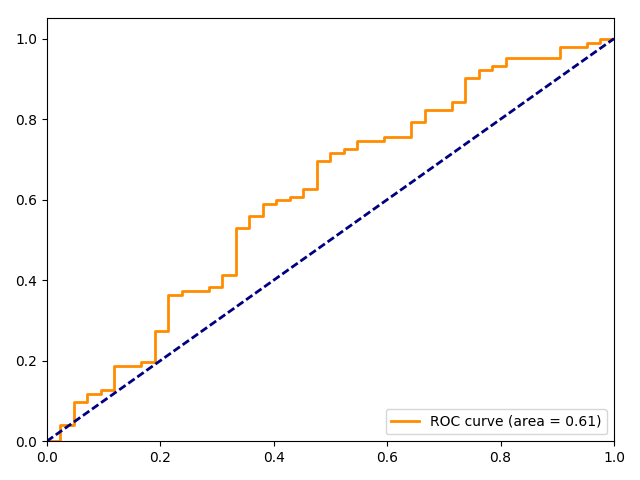
\includegraphics[width=0.7\textwidth]{./img/max_on_circle.png}
\end{center}
\caption{Wynik działania deskryptora, AUC.}
\end{figure}


\subsection{Porównanie jasności punktów}
\subsubsection{Ekstrakcja}
Metoda opiera się na algorytmie BRIEF z modyfikacjami. Przy inicjacji algorytmu jest losowancyh 512 punktów należących do okręgu o wielkości rozważanego deskryptora z jednostajnym prawdopodobieństwem.

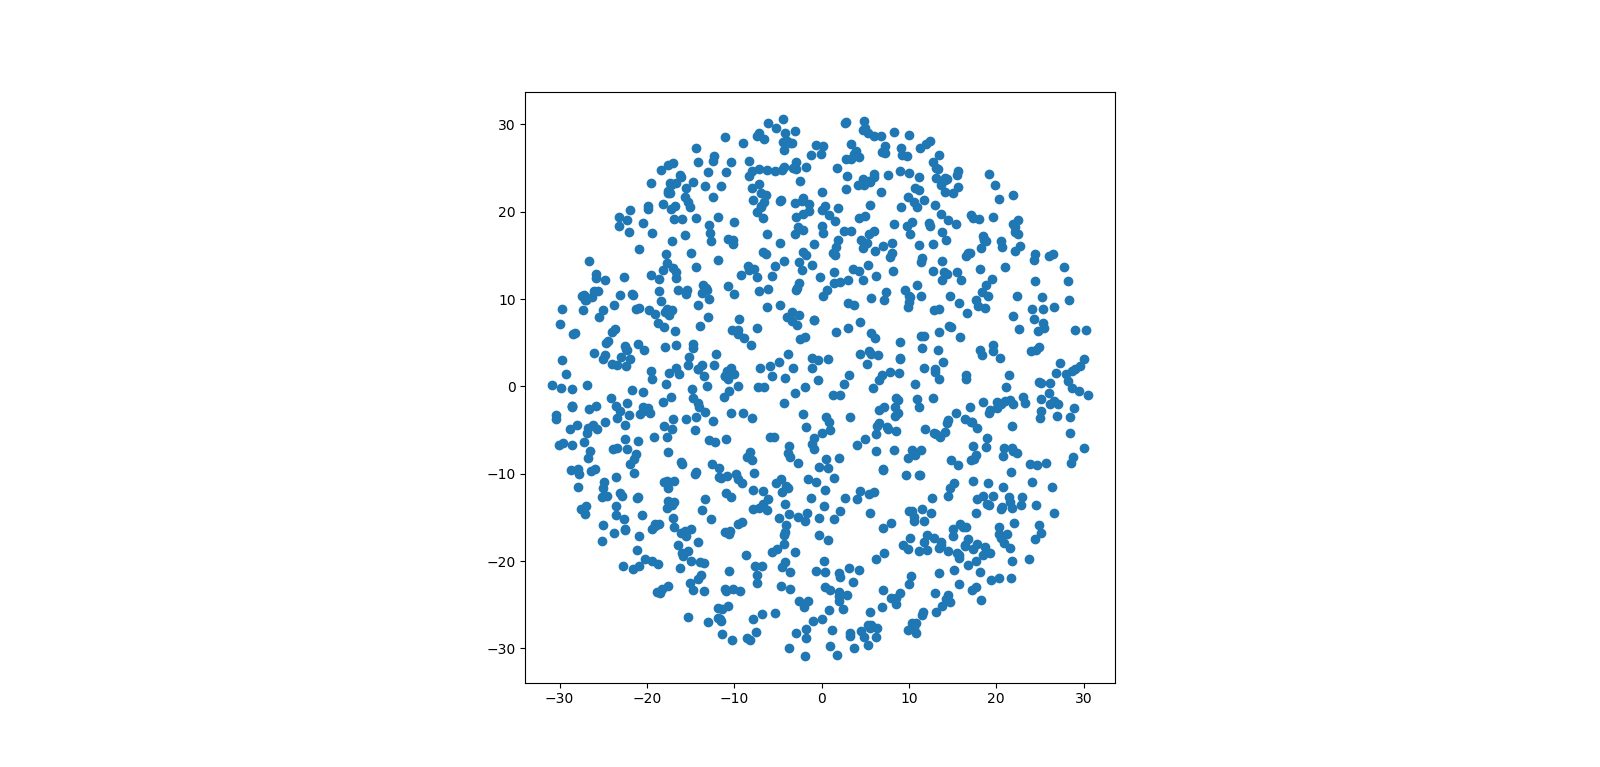
\includegraphics[width=0.7\textwidth]{./img/points.png}

Dla otoczenia punktu jest obliczany kąt oraz długość gradientu dla każdego z piksela. Używany jest do tego pionowy i poziomy filtr Sobela -- $g_x$ oraz $g_y$, a następnie gradient jest obliczany ze wzoru:

$$ g = \sqrt{g_x^2 + g_y^2}$$
$$ \theta =arctan \frac{g_y}{g_x}$$

Z wyliczonych wartości jest obliczany dominujący gradient z kątów $\theta$ przy pomocy średniej wazonej z wagami $g$. Nastepnie obraz jest obracany wg tego gradientu. W kolejnymkorku są porównywane jasności punktów parami. Jeżeli jasność pierwszegopunktu jest większa niż drugiego to do deskryptora jest zapisywana wartość 1, 0 w przeciwnym przypadku. Lista 0 i 1 tworzy deskryptor.

\section{Porównanie}

Porównanie deskryptorówpolega na obliczenieniu ich odległości Hamminga.

\subsection{Porównanie}
Porównywanie obrazów odbywa się przy pomocy odległości Hamminga.


\subsubsection{Wynik działania}

\begin{figure}[H]
\begin{center}
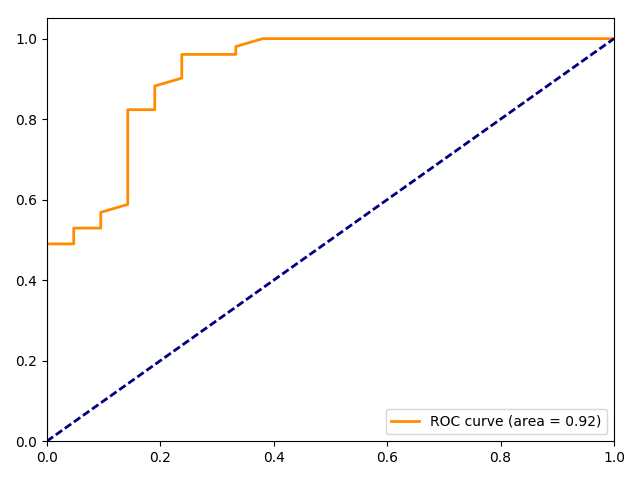
\includegraphics[width=0.7\textwidth]{./img/brief.png}
\end{center}
\caption{Wynik działania deskryptora, AUC.}
\end{figure}

\section{Testowanie}
Aby móc dobrze ocenić działanie deskryptora zostały napisane dwa skrypty umożliwiające sprawdzenie jakości naszego rozwiązania. Pierwszy używa prawdziwych zdjęć z podanego zbioru losując punkty i zapisując ich współrzędne wraz z odpowiadającymi im punktami w odpowiadających zdjęciach. Drugi zaś wybiera losowy fragment i poddaje go transformacją:
\begin{enumerate}
\item rozmycia,
\item korekcji gamma,
\item obrotowi,
\item powiększeniu,
\item kompresji jpg.
\end{enumerate}

\end{document}  
